\documentclass{article}%
\usepackage[T1]{fontenc}%
\usepackage[utf8]{inputenc}%
\usepackage{lmodern}%
\usepackage{textcomp}%
\usepackage{lastpage}%
\usepackage[head=40pt,margin=0.5in,bottom=0.6in]{geometry}%
\usepackage{graphicx}%
%
\title{\textbf{Sindicatos de salud de Nueva Esparta se suman a la "toma nacional" de la sede ministerial}}%
\author{ANA CAROLINA ARIAS}%
\date{19/09/2018}%
%
\begin{document}%
\normalsize%
\maketitle%
\textbf{URL: }%
http://www.eluniversal.com/venezuela/21088/sindicatos{-}de{-}salud{-}de{-}nueva{-}esparta{-}se{-}suman{-}a{-}la{-}toma{-}nacional{-}de{-}la{-}sede{-}ministerial\newline%
%
\textbf{Periodico: }%
EU, %
ID: %
21088, %
Seccion: %
venezuela\newline%
%
\textbf{Palabras Claves: }%
NO\_TIENE\newline%
%
\textbf{Derecho: }%
2.1, %
Otros Derechos: %
, %
Sub Derechos: %
2.1.1\newline%
%
\textbf{EP: }%
SI\newline%
\newline%
%
\textbf{\textit{Trabajadores protestaron por el incumplimiento de la contratación colectiva a raíz de la nueva política salarial}}%
\newline%
\newline%
%
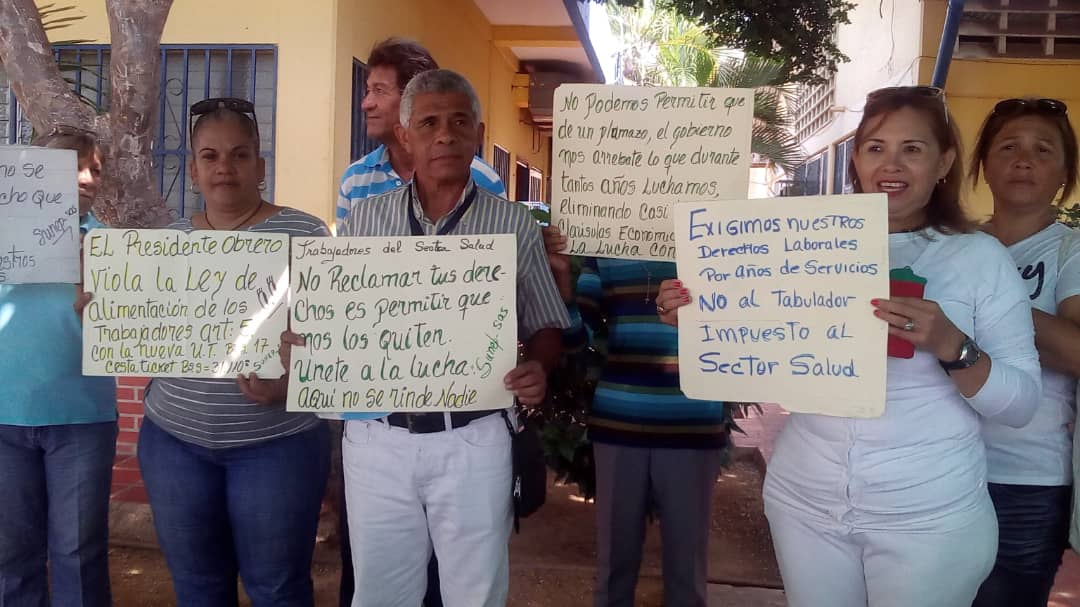
\includegraphics[width=300px]{81.jpg}%
\newline%
%
Porlamar.{-} Agremiados al Sindicato de Trabajadores de la Salud en el estado Nueva Esparta (Sunep{-}SAS) se sumaron este martes al llamado a tomas nacionales de los centros asistenciales y administrativos del Ministerio de la Salud, y acordaron declararse en emergencia hasta que el Gobierno nacional de una "respuesta efectiva" a la nueva política de pago nacional.%
\newline%
%
La posición es de absoluto rechazo al tabulador salarial que está aplicando el Gobierno a todos los sectores, incluyendo la salud. "Exigimos nuestros derechos laborales por años de servicio". "El presidente obrero (Nicolás Maduro) viola la Ley de Alimentación  de los trabajadores  ante la nueva UT", expresaron en los carteles exhibidos.%
\newline%
%
Emilio Serra, secretario general del referido ente sindical, fue el vocero de la concentración que se llevó a cabo en la sede de la Dirección Regional de Salud, explicando que el nuevo salario mínimo nacional “eliminó de un plumazo” todos los beneficios laborales alcanzados hasta ahora por los gremios.%
\newline%
%
“La práctica eliminación que se está haciendo de los contratos colectivos es violatoria del derecho a la progresividad que tantos años hemos luchado, y no sabemos hasta dónde pretende llegar el Gobierno, porque ha tumbado lo más sagrado para los trabajadores que son sus reivindicaciones conseguidas en años de lucha”.%
\newline%
%
Rechazo a monto del cestaticket%
\newline%
%
Específicamente, dijo que es grave la falta al artículo 5 de la Ley de Alimentación, que estipula que el bono por este concepto no puede ser inferior al 0,25\% de la unidad tributaria, “si ahora tenemos una Unidad Tributaria fijada en 17 bolívares soberanos, la cestaticket debe estar en tres mil 110 bolívares soberanos y lo que nos están pagando es el 10\% del salario mínimo, es decir 180 bolívares soberanos”.%
\newline%
%
Ante lo que califican como “serios atropellos”, Serra hizo un llamado a todos los trabajadores para que apoyen las acciones de protesta, anunciando de hecho que trabajadores de otros ministerios también declararán el conflicto porque no aceptarán que, “quien dice llamarse un presidente obrero elimine de un solo golpe lo que con tantos sacrificios hemos logrado alcanzar”.%
\newline%
%
\end{document}